\item[17] More CPU functions \\
\textit{Comparison} is an important operation which a CPU needs to perform. It is a critical feature that allows us to write conditional branches in programs executed on this CPU. Logisim provides a \textit{comparator} component in its arithmetic library - in this exercise we will construct our own components to perform arithmetic comparison between two unsigned integer inputs.

  We will begin our construction with a 1-bit comparator, described as follows: \\

     \begin{itemize}
      \item 1-bit inputs: $a$, $b$, $cl$, $cg$
      \item 1-bit outputs: $gt$, $eq$, $lt$
     \end{itemize}
     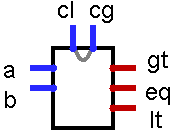
\includegraphics[height=1.8cm]{compare-1-pkg.png} \\

    For multi-bit comparison between two $n$-bit unsigned values $A=a_{n-1}\ldots a_{0}$ and $B=b_{n-1}\ldots b_{0}$, $gt=1$ if $A>B$, $eq=1$ if $A=B$, $lt=1$ if $A<B$, and only one of $gt$, $eq$, and $lt$ will be active. For single-bit comparison, $cl$ and $cg$ must be considered - these receive information about the comparison result of the bit(s) to the right of the current bit being compared. For example, suppose we are comparing bit 1 of $A=10$ and $B=11$ - what should the output be, assuming that bit 0 has already been compared, and $a_1=b_1$?

\begin{question}{a.}[3]
  \item[5] Complete the function table for the 1-bit comparator, based on your understanding of the description above. Some rows have already been completed for you. For the comparison of some bit $i$, is it possible for the result from bits $i-1 \ldots 0$ to be both greater than \textit{and} less than?
  
  \begin{tabular}{c c c c | c c c}
    $a$ & $b$ & $cl$ & $cg$ & $gt$ & $eq$ & $lt$ \\
    \hline
    0 & 0 & 0 & 0 & 0 & 1 & 0 \\
    0 & 0 & 0 & 1 &  &  &  \\
    0 & 0 & 1 & 0 &  &  &  \\
    0 & 0 & 1 & 1 &  &  &  \\
    \hline
    0 & 1 & 0 & 0 & 0 & 0 & 1 \\
    0 & 1 & 0 & 1 &  &  &  \\
    0 & 1 & 1 & 0 &  &  &  \\
    0 & 1 & 1 & 1 &  &  &  \\
    \hline
    1 & 0 & 0 & 0 & 1 & 0 & 0 \\
    1 & 0 & 0 & 1 &  &  &  \\
    1 & 0 & 1 & 0 &  &  &  \\
    1 & 0 & 1 & 1 &  &  &  \\
    \hline
    1 & 1 & 0 & 0 & 0 & 1 & 0 \\
    1 & 1 & 0 & 1 &  &  &  \\
    1 & 1 & 1 & 0 &  &  &  \\
    1 & 1 & 1 & 1 &  &  &  \\
  \end{tabular}
  
  \newpage
  
  \item[8] For this question, please refer to the Logisim User's Guide, section "Subcircuits" - "Creating circuits", and "Using subcircuits". In Logisim, choose "Project -> Add Circuit", and call the new circuit "comparator-1". In the drawing area for your comparator-1 component, use no more than 13 logic gates \textit{in total} to design a circuit which implements the behaviour of this 1-bit comparator. Your solution should produce all of the three required outputs on a single circuit.
  
  Your circuit diagram here:
  
  \vspace{10.0cm}
  
  \item[4] For this question, you will use the subcircuit for comparator-1 produced in the previous question. In the drawing area for your main circuit, use four (4) copies of your comparator-1 component, and any other gates necessary, as well as power/constant-1 and ground/constant-0, to construct a 4-bit unsigned comparator. Connect 4-bit inputs $A$ and $B$ (by setting data width to 4) and test your circuit. You will need to use splitters to access the individual bits of your 4-bit inputs.
  
  Your circuit diagram here:
  
  \vspace {6.0cm}
  
\end{question}

\newpage

